\documentclass[../main/main.tex]{subfiles}

\begin{document}

\section{Линейные радиотехнические цепи.}

\subsection{Условие квазистационарности.}
В общем случае электрические сигналы, проходя по цепям, изменяются во времени: 
$$i = i(t),~u=u(t),~\Phi = \Phi(t)~\text{и т.д.}$$

В окружающем пространстве имеется электромагнитное поле в виде электромагнитной волны, возникающей при переменных токах, зарядах и др. Волны несут информацию об "изменениях"\ в соседних точках цепи, что описывается функциями вида
$$f = f\bigg(t - \dfrac{x}{v}\bigg),$$
где $v$ --- скорость электромагнитной волны в данной среде, $x$ --- пространственная координата. Пусть $\tau_0$ --- характерное время изменения сигнала. Тогда, если $x~\ll~v\tau_0$ ($0\leqslant x \leqslant L$), во всех точках приближенно можно считать функцию $f(t, x)$ одинаковой, т.е. независимой в данный момент момент $t$ от координаты $x$: 
$$f(t, x) \bigg|_{x=0} \simeq f(t, x)\bigg|_{x=vt}\simeq f(t).$$

Другими словами, мы пренебрегаем эффектами запаздывания. Если $L$ --- характерный размер цепи, тогда потребуется:
$$x_{max} = L \ll v\tau_0 = \lambda~\text{(для гармонического сигнала: }~\tau_0=\dfrac{2\pi}{\omega})$$
и "условие квазистационарности": 
\begin{center}
$\boxed{L \ll \lambda}$ или $\dfrac{\tau}{\tau_0} \ll 1$,
\end{center}
где $\tau$ --- время передачи информации.

Цепи, удовлетворяющие этому условию, называются \underline{сосредоточенными цепями}. Пример: $\nu = 50$ Гц, $\lambda = c/\nu \simeq 6\cdot10^3$ км. Любая более короткая линия может считаться "сосредоточенной". Это, конечно, следствие низкой частоты.

\subsection{Линейные элементы цепей.}

Общим свойством простых сосредоточенных цепей является "линейность", т.е. подчинение принципу суперпозиции: реакция цепи на суммарный сигнал равна сумме реакций на каждый из сигналов в отдельности. Элементами таких цепей будут: сопротивление (резисторы), емкость (конденсаторы), индуктивность (катушки).

\begin{enumerate}
    \item Сопротивление $R$.
    
\begin{minipage}{6cm}
\centering
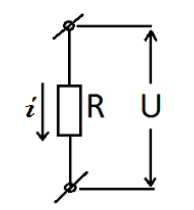
\includegraphics[scale=0.7]{../section01/images/resistor/resistor.png} % нужна картинка
\end{minipage} \hfill   
\begin{minipage}{11cm}
Также вводится понятие проводимости $G = \dfrac{1}{R}$. Размерности $R = [\text{Ом}],~G = [\text{Ом}^{-1}]$. Связь тока, напряжения и сопротивления (закон Ома): $i=\dfrac{U}{R}=GU$. $P=Ui$ --- мощность. $\Delta W_R = \displaystyle \int \limits_{0}^{t} Ui \, dt$ --- энергия, выделяемая на резисторе за время от $0$ до $t$.
\end{minipage}
    
    По отношению к реальным сопротивлениям --- это идеализация. Предполагается, что нет зависимостей $R(i)$ или $R(U)$ (в ином случае можно говорить о локальных $R$ и $G$ в окрестности точки $i = \text{const}$, их называют "дифференциальными"\ характеристиками: $R_\partial = \dfrac{dU}{di}\bigg|_{i=0},~G_\partial = R_\partial^{-1}$). На практике зависимость $R(i)$ может возникнуть, благодаря температурной вариации сопротивления $R(T)$: рост тока сопровождается нагревом и изменением $R$. Обычно на резисторе указывается предельно допустимая мощность, ниже которой "линейность"\ c заданной точностью гарантируется.
    
    \item Ёмкость $C$. 

\begin{minipage}{6cm}
\centering
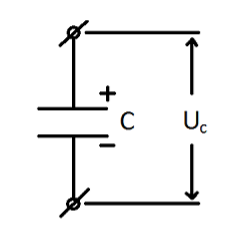
\includegraphics[scale=0.7]{../section01/images/capacitor/capacitor.png} % нужна картинка
\end{minipage} \hfill   
\begin{minipage}{11cm}
    Заряд $q = CU_C$. "Ток смещения": $i = \dfrac{dq}{dt} = C \dfrac{dU_C}{dt}$. Энергия, выделяемая за время от $0$ до $t$: $W_C = \dfrac{1}{C} \displaystyle \int\limits_{0}^{t} i \, dt$. Вариация энергии: $\Delta W_C = W_C(t) - W(0) = \dfrac{C}{2} [U_C^2(t) - U_C^2(0)]$.
\end{minipage}


    
    Здесь также предполагается $C = \text{const}$, т.е. нет зависимости $C(U)$. Примеры, когда это не выполняется: конденсатор с сегнетоэлектриком, pn-переход и др. Если $C = C(U)$, то при $U = U_0 = \text{\text{const}}$ вводят $C_\partial = \dfrac{dq}{dU}$. 
    
\begin{minipage}{6cm}
\centering
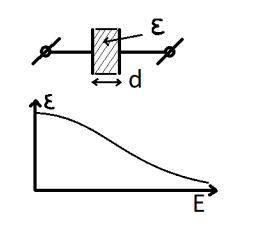
\includegraphics[scale=0.7]{../section01/images/capacitor_plot/capacitor_plot.png} % нужна картинка
\end{minipage} \hfill   
\begin{minipage}{11cm}
    $\varepsilon = \dfrac{\varepsilon(0)}{1 + \bigg(\dfrac{\varepsilon(0)}{4\pi}\bigg)^3 BE^2}$ --- постоянная материала, где $B = \text{\text{const}}$, $E$ --- электрическое поле. Тогда, $C_U = \dfrac{C(0)}{1 + bU^2}$. В линейных системах эти эффекты опускаются. 
\end{minipage}
    
    \item Индуктивность $L$.
    
\begin{minipage}{6cm}
\centering
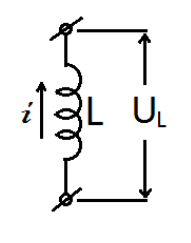
\includegraphics[scale=0.6]{../section01/images/inductance/inductance.png} % нужна картинка
\end{minipage} \hfill   
\begin{minipage}{11cm}
    Магнитный поток $\Phi = Li$. Напряжение $U = \dfrac{d\Phi}{dt} = L \dfrac{di}{dt}$. Выделяемая энергия на элементе $W_L = \dfrac{1}{2} Li^2$. Вариация энергии $\Delta W_L = \dfrac{L}{2} [i^2(t) - i^2(0)]$.
\end{minipage}
    
    Для этого элемента также возможно $L = L(i)$. Например, для катушки с сердечником $\mu = \mu(i) \Rightarrow L_\partial = \dfrac{d\Phi}{di}$.
\end{enumerate}

\subsection{Источники энергии.}

Это тоже элементы радиотехнических цепей: постоянные(батареи, аккумуляторы), переменные(генераторы). Эквивалентная схема источника должна содержать его внутреннее сопротивление.
 
\begin{minipage}{6cm}
\centering
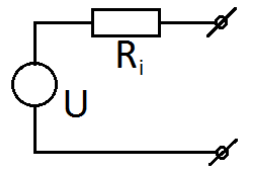
\includegraphics[scale=0.7]{../section01/images/not_ideal_voltage/not_ideal_voltage.png} % нужна картинка
\end{minipage} \hfill   
\begin{minipage}{11cm}
Здесь известны два предельных случая ("две абстракции"\ или "идеализации"):
\end{minipage}

\begin{enumerate}
    \item Генератор тока (идеальный источник тока).
        Внутреннее сопротивление велико по сравнению с сопротивлением внешней цепи (нагрузки): $R_i \gg R (G_i \rightarrow 0)$. Тогда, $i = \dfrac{U}{R_i + R} \simeq \dfrac{U}{R_i} = \text{const}$ --- т.е. ток не зависит от $R$! (источник снабжает нагрузку фиксированным током). 
    
    \item Генератор напряжения (идеальный источник напряжения).
     Внутреннее сопротивление мало по сравнению с сопротивлением внешней цепи: $R_i \ll R (R_i \rightarrow 0)$. Тогда, $i \simeq \dfrac{U}{R}$ или $U \simeq iR = U_0$ (напряжение, создаваемое во внешней цепи не зависит от нагрузки).  
\end{enumerate}

Реальные источники только приближенно могут быть отнесены к одному из этих генераторов.

\subsection{Уравнения простейших линейных цепей.}

Рассмотрим подробно $RC$-цепь.

\begin{minipage}{6cm}
\centering
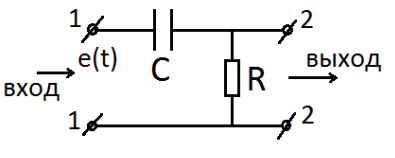
\includegraphics[scale=0.6]{../section01/images/rc_simple/rc_simple.png} % нужна картинка
\end{minipage} \hfill   
\begin{minipage}{9cm}
Пусть~входной сигнал содержит постоянную и~переменную составляющую: $e(t) = U_0 +~U(t)$. Тогда: $e(t) = U_C + U_R \Rightarrow U_C = \dfrac{1}{C} \displaystyle \int i \, dt,\\U_R = iR,\quad i=\dfrac{dq}{dt} = C \dfrac{dU_C}{dt} \Rightarrow\\e(t) = U_C + RC\dfrac{dU_C}{dt}$ --- дифференциальное уравнение относительно $U_C$. 
\end{minipage}

Нас интересует вид выходного сигнала (обозначения: $RC = \tau_0,~\dfrac{t}{\tau_0} = \tau$). Решать следует обычными методами из теории дифференциальных уравнений. % в книге \tau потом нигде не используется, я записал уравнения с ней.

Домножим уравнение на $e^\tau$:
$$e(t) e^\tau = U_C e^\tau + \tau_0 e^\tau \dfrac{dU_c}{d\tau} = \dfrac{d}{dt}\bigg( \tau_0 U_C e^\tau \bigg),$$
$$d \bigg( \tau_0 U_C e^\tau \bigg) = e(t) e^\tau dt.$$

Простым интегрированием и переносом множителей получим: 
$$U_C = \frac{1}{\tau_0} e^{-\tau} \displaystyle \int\limits_0^t e(t) e^{\tau} dt +  \text{const} \cdot e^{-\tau}$$

Добавим начальные условия, например: $t = 0,~U_C = 0$, тогда $\text{const} = 0$.

\underline{На входе постоянный сигнал $e(t) = U_0$.}

\begin{minipage}{6cm}
\centering % я убрал картинку с постоянным напряжением, т.к. и так очевидно как оно выглядит
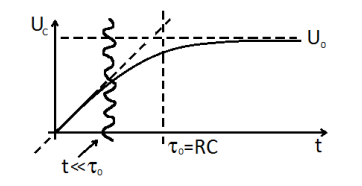
\includegraphics[scale=0.6]{../section01/images/U_C_plot/U_C_plot.png} % нужна картинка
\end{minipage} \hfill   
\begin{minipage}{9cm}
Очевидно, $U_R = e(t) - U_C(t)$, из формулы получим $U_C = U_0 (1 - e^{-\tau}) \rightarrow U_R = U_0 e^{-\tau}$. Рассмотрим здесь 2 области: 

\begin{enumerate}
\item $t \ll \tau_0,~U_C \sim t,~U_R \sim U_0 \dfrac{t}{RC}$. Это "область интегрирования", сигнал снимается с ёмкости. Видно запаздывание напряжения по откошенной по току на время $\tau_0 = RC$.
\end{enumerate}
\end{minipage}

\begin{minipage}{6cm}
\centering
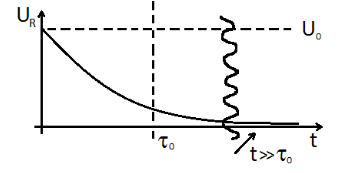
\includegraphics[scale=0.6]{../section01/images/U_R_plot/U_R_plot.png} % нужна картинка
\end{minipage} \hfill   
\begin{minipage}{9cm}
\begin{enumerate}
\setcounter{enumi}{1}
\item $t \gg \tau_0,~U_R = U_0 e^{-\tau} \simeq 0$. Это "область дифференцирования", сигнал снимается с сопротивления. Для гармонического сигнала это приводит к разности фаз $\sim \pi / 2$ между $U_{\text{вх}}$ и $U_{\text{вых}}$. 
\end{enumerate}
\end{minipage}

Графики $U_C(t)$ и $U_R(t)$ показывают, что можно использовать радиотехнические цепи для выполнения математических операций интегрирования и дифференцирования (в аналоговой форме). Все зависит от соотношения длительности входного сигнала и постоянной времени цепи $\tau_0$:

\begin{enumerate}
\item Дифференцируемая $RC$-цепочка.

\begin{minipage}{6cm}
% \centering
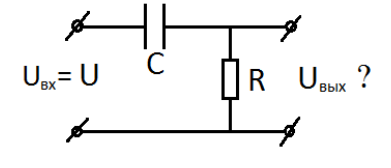
\includegraphics[scale=0.5]{../section01/images/R_C_derivate/R_C_derivate.png} % нужна картинка
\end{minipage} \hfill   
\begin{minipage}{9cm}
$U_{\text{вых}} = U_R = R \cdot C\dfrac{dU_c}{dt} = RC\bigg(\dfrac{dU_\text{вх}}{dt} - \dfrac{dU_R}{dt}\bigg)$. Если $\dfrac{dU_R}{dt} \ll \dfrac{dU}{dt}$, тогда $U_\text{вых} = U_R \simeq \tau_0 \dfrac{dU}{dt} \Rightarrow$ цепочка будет дифференцировать сигнал.
\end{minipage}

$$\dfrac{dU_R}{dt} \ll \dfrac{dU}{dt} \sim \dfrac{U_R}{RC},~\text{т.е.}~\dfrac{RC}{U_R} \dfrac{dU_R}{dt} \ll 1~\text{или}~\boxed{\dfrac{\tau_0}{\tau_C} \ll 1},$$
где $\dfrac{1}{U_R} \dfrac{dU_R}{dt} \sim \frac{1}{\tau_C}$ --- обратная длительность сигнала.

\item Интегрирующая $RC$-цепочка.

\begin{minipage}{6cm}
\centering
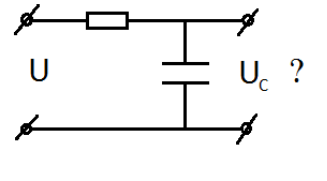
\includegraphics[scale=0.6]{../section01/images/R_C_integrate/R_C_integrate.png} % нужна картинка
\end{minipage} \hfill   
\begin{minipage}{9cm}
$U = \dfrac{1}{RC} \displaystyle \int\limits_0^t U \, dt = U \dfrac{t}{RC} \Rightarrow$ цепочка интегрирует входной сигнал. Для интегрирующей цепочки~$\tau_0 \gg \tau_C$.
\end{minipage}
\end{enumerate}

Для гармонического сигнала характерное время $\tau_C \simeq \dfrac{2\pi}{\omega}$, условия дифференцируемости и~интегрируемости переписываются в виде:
$$\text{дифф. цепь} \quad \tau_0 \ll \tau_C \rightarrow \dfrac{\omega RC}{2\pi} \gg 1;$$
$$\text{интегр. цепь} \quad \tau_0 \gg \tau_C \rightarrow \dfrac{\omega RC}{2\pi} \ll 1.$$

\textbf{Упражнение 1.} Построить аналогичные цепочки из элементов $L$ и $C$ и рассчитать реакцию на ступенчатый импульс.

Общий вывод следующий: Видно, что уже с помощью линейных инерционных элементов радиотехнических цепей можно выполнять существенные операции математического анализа. Добавление нелинейных элементов, конечно, расширит возможности. Здесь ключ к пониманию принципов построения аналоговых вычислительных машин.

Метод анализа процессов в радиотехнических цепях с помощью решения дифференциальных уравнений полон (описывает как стационарные состояния, так и переходные режимы), но не слишком прост. На практике техниками, радиоинженерами, радиолюбителями и др. используется (без строгого обоснования) "метод комплексных амплитуд"{} (МКА).
 
\subsection{Метод комплексных амплитуд (МКА).}

Качественное обоснование метода следующее: гармонический сигнал представляется в~комплексной форме: 
$$U(t) = U_0 \cos(\omega t + \varphi) = \dfrac{U_0}{2}(e^{j(\omega t + \varphi)} + e^{-j(\omega t + \varphi)}) = \widetilde{U} e^{\jo t} + \text{к.с.},$$
где $\widetilde{U} = \dfrac{U_0}{2} e^{j \varphi}$ --- "комплексная амплитуда"{} сигнала.

В~силу принципа суперпозиции можно рассчитать реакцию цепи на~"комплексный сигнал"{}~$\widetilde{U} e^{\jo t}$ и~к~результату прибавить комплексно-сопряженное решение (если нас интересует временная зависимость выходного напряжения в явной форме; часто, однако, этого не~требуется). Если это принять, то отпадает необходимость в~решении дифференциальных уравнений при~расчете цепей. Действительно: дифференциальные соотношения при~этом превращаются в~алгебраические. Введём напряжение сигнала $U = \widetilde{U} e^{\jo t}$. Тогда рассмотрим: 
\begin{enumerate}
\item Ток через~резистор: $i = \dfrac{U}{R} = \widetilde{i}_0 e^{\jo t},~\widetilde{i}_0 = \dfrac{\widetilde{U}}{R}$ --- комплексная амплитуда тока, фаза не~изменилась;

\item Ток через ёмкость: $i = C \dfrac{dU_C}{dt} = \jo C \widetilde{U} e^{\jo t} = \dfrac{\widetilde{U}}{1/(\omega C)} e^{j\bigg(\omega t + \dfrac{\pi}{2}\bigg)}$ --- ток через~ёмкость опережает напряжение на~$\varphi = \dfrac{\pi}{2}$. Тогда, ток~будет равен:~$\widetilde{i} = \dfrac{\widetilde{U}}{|X_C|}$, где~$X_C = \dfrac{1}{\jo C}$ --- комплексное сопротивление ёмкости. 

При~$\omega \rightarrow 0$ получим $X_C \rightarrow \infty$ --- постоянный ток не~течёт. 

При~$\omega \rightarrow \infty,~|X_C| \rightarrow 0$ --- короткое замыкание на~высоких частотах.

\item Ток через~индуктивность: $U = \widetilde{U} e^{\jo t}, i = \frac{\Phi}{L} = \displaystyle \int U \, dt \Rightarrow i = \dfrac{1}{\jo L \widetilde{U} e^{\jo t}} = \dfrac{\widetilde{U}}{\omega L} e^{j\bigg(\omega t - \dfrac{\pi}{2}\bigg)}$ --- ток через~индуктивность отстаёт от~напряжения на~$\varphi = \dfrac{\pi}{2}$. Тогда, ток будет~равен:~$\widetilde{i}~=~\dfrac{\widetilde{U}}{|X_L|}$, где $X_L = \jo L \rightarrow |X_L| = \omega L$ --- комплексное сопротивление индуктивности.

При~$\omega \rightarrow 0$ получим $i \rightarrow \infty$ --- отсутствие сопротивления постоянному току. 

При~$\omega \rightarrow \infty,~\widetilde{i} \rightarrow 0$ --- "разрыв"{} цепи на~высоких частотах.

\end{enumerate}

\subsection{Расчет цепей методом комплексных амплитуд.}

Исследуем методом комплексных амплитуд $RC$-цепь.

\begin{minipage}{6cm}
\centering
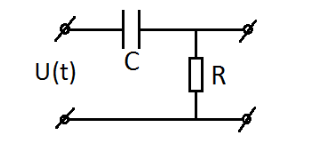
\includegraphics[scale=0.7]{../section01/images/RC_MKA/RC_MKA.png} % нужна картинка
\end{minipage} \hfill   
\begin{minipage}{10cm}
Напряжение $U = U_C + RC \dfrac{dU_C}{dt}$ \textit{(см. п.4)}.

Представим входной сигнал в комплексной форме $U(t) = U_0 e^{\jo t}$ ($U_0$ --- действительная амплитуда), $U_C = \widetilde{U_C} e^{\jo t}$.

Подстановка даёт $U_0 = \widetilde{U_C} + \jo RC \widetilde{U_C}$ (т.е. дифференциальное уравнение перешло в алгебраическое). Выражая, получим: 
\end{minipage}

$$\widetilde{U_C} = \dfrac{U_0}{1 + \jo RC}, \quad \widetilde{U_R} = U_0 - \widetilde{U_C} = \dfrac{\jo RC U_0}{1 + \jo RC}.$$

Эти же формулы можно получить, используя закон Ома и законы Кирхгофа с $R_C \rightarrow X_C = \dfrac{1}{\jo C}$: 
$$\widetilde{i_0} = \dfrac{U_0}{R + \dfrac{1}{\jo C}}, \quad \widetilde{U_R} = \widetilde{i_0} R = \dfrac{\jo RC U_0}{1 + \jo RC}.$$

Проанализируем результат: 
$$\widetilde{U_R} = \dfrac{\jo RC}{1 + \jo RC} U_0~\text{выразим в виде:}~\widetilde{U_R} = \dfrac{U_0}{|Z(\omega)|}e^{j \varphi},$$
$$|Z(\omega)| = \bigg| \dfrac{\jo RC}{1 + \jo RC} \bigg| = \dfrac{\omega RC}{\sqrt{1 + (\omega RC)^2}}$$

\begin{minipage}{6cm}
\centering
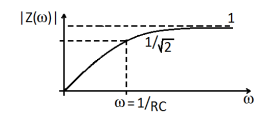
\includegraphics[scale=0.7]{../section01/images/Z_o_plot/Z_o_plot.png} % нужна картинка
\end{minipage} \hfill   
\begin{minipage}{10cm}
$|Z(\jo)| = |K(\jo)| = \bigg| \dfrac{\widetilde{U_R}}{U_0} \bigg|$.

Получаем "завал"{} коэффициента предачи на низких частотах.
\end{minipage}

"Коэффициент передачи"{} $|K(\jo)|$, он же --- "Амлитудно-чатотная характеристика"{} радиотехнической цепи. 

Также, существует "фазо-частотная характеристика"{} $\varphi(\omega)$: 
$$\tan \varphi(\omega) = \dfrac{\text{Im} Z(\jo)}{\text{Re} Z(\jo)},$$
$$Z(\omega) = \dfrac{\jo RC}{1 + \jo RC} \quad \rightarrow \quad \varphi(\omega) = \arctan \bigg( \dfrac{1}{\omega RC} \bigg)$$

\begin{minipage}{6cm}
\centering
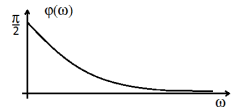
\includegraphics[scale=0.7]{../section01/images/phi_o_plot/phi_o_plot.png} % нужна картинка
\end{minipage} \hfill   
\begin{minipage}{10cm}
На высоких частотах фазовое "искажение"{} исчезает.
\end{minipage}

Таким образом, мы провели "частотный анализ"{} прохождения переменного сигнала через $RC$-цепочку.

\textbf{Упражнение 2.} Выполнить тоже самое для сигнала, снимаемого с емкости, т.е. изучить $U_C$.

В общем случае, для произвольной линейной цепи, следует ожидать, что:
$$\widetilde{U}_\text{вых} (\jo) = \widetilde{U}_\text{вх} \widetilde{K}(\jo); \quad \widetilde{K}(\jo) = |\widetilde{K}(\jo)| e^{j \varphi(\omega)},$$
т.е. прохождения сигнала через радиотехническую цепь описывается на языке, типичном для "задачи рассеяния".

\subsection{Метод преобразования Лапласа. Расчёт переходных режимов.}

Данный способ более мощный, чем МКА и позволяет описывать не только стационарные, но и переходные процессы в радиотехнических цепях.

Покажем метод Лапласа на примере $RC$-цепи \textit{(см. п.6)}:
$$e(t) = R i(t) + \dfrac{1}{C} \displaystyle \int i(t) \, dt.$$
Формальное определение преобразования Лапласа: 
$$f(t) \rightarrow \widehat{f} (p) = \displaystyle \int\limits_0^\infty f(t) e^{-pt} \, dt$$
Обратным преобразованием Лапласа называется: 
$$\widehat{f}(p) \rightarrow f(t) = \dfrac{1}{2\pi i} \displaystyle \lim\limits_{r\rightarrow \infty} \int\limits_{\delta - ir}^{\delta + ir} f(p) e^{-pt} \, dp,$$
параметр $p = \delta + i\omega$ --- комплексное число.

Существуют таблицы $f(t) \leftrightarrows \widehat{f}(p)$ для типичных функций. Кроме того, известны свойства преобразования Лапласа: 
$$\alpha f_1(t) + \beta f_2(t) \Rightarrow \alpha \widehat{f_1}(p) + \beta \widehat{f_2}(p)$$
$$\dot{f(t)} \Rightarrow p \widehat{f}(p) - f(0+0)$$
$$\displaystyle \int\limits_0^\infty f(t) dt \Rightarrow \dfrac{f(p)}{p}$$
$$f(at) \Rightarrow \dfrac{1}{a}\widehat{f}(\dfrac{p}{a}),~a>0$$
$$f(t-b) \Rightarrow r^{bp} \widehat{f}(p)~\text{и др.}$$
После преобразования уравнения $RC$-цепи получим: 
$$\widehat{e}(p) = \bigg(R + \dfrac{1}{pC}\bigg) \widehat{i}(p),~ Z_C(p) = \dfrac{1}{pC}.$$
Для постоянного тока:

\begin{equation*}
e(t) = 
 \begin{cases}
   u_0, &t \geq 0\quad\quad \longrightarrow \quad \widehat{e}(p) = \dfrac{u_0}{p} \\ 
   0, &t < 0
 \end{cases}
\end{equation*}

Тогда:
$$\widehat{i}(p) = \dfrac{\widehat{e}(p)}{R + \dfrac{1}{pC}},$$
$$\widehat{U_R} = R\widehat{i}(p) = \dfrac{u_0}{p + \dfrac{1}{\tau_0}},~\tau_0 = RC,$$
$$\widehat{U_C} = Z_C(p) \widehat{i}(p) = \dfrac{u_0}{p\tau_0 (P + \dfrac{1}{\tau_0})}$$

Из обратного преобразования Лапласа (по таблицам) получим: 
$$U_R = U_0 e^{-t/\tau_0}, \quad U_C = U_0 (1 - e^{-t/\tau_0}) \textit{см. п.4}.$$
Сейчас можно ввести понятие "передаточной функции"{} $H(p)$: 
$$\widehat{U_R} = H_R \widehat{e(p)}~\Rightarrow~H_R(p) = \dfrac{\widehat{U_R}}{\widehat{e}};$$
$$H_R(p) = \dfrac{p}{p + \dfrac{1}{\tau_0}}, \quad p = \delta + \jo.$$
При $\delta \rightarrow 0$, $H_R$ переходит в частотную характеристику \textit{(см. п.6)}.

$$H_R (\jo) = \dfrac{\widehat{U}_R(\jo)}{\widehat{e}(\jo)} = \widetilde{K_R} (\jo) = \dfrac{\jo \tau_0}{1 + \jo \tau_0}\rightarrow \jo \tau_0~(\text{для дифф. цепи, т.к. } \omega \tau_0 \ll 1;$$
$$H_C (\jo) = \dfrac{\widehat{U}_C(\jo)}{\widehat{e}(\jo)} = \widetilde{K_C} (\jo) = \dfrac{1}{1 + \jo \tau_0} \rightarrow \frac{1}{\jo \tau_0}~(\text{для интегр. цепи, т.к. } \omega \tau_0 \gg 1.$$

\textbf{Упражнение 3.} Получите аналогичные выражения для $LC$-цепи.

\subsection{Последовательный колебательный контур.}

\begin{minipage}{6cm}
\centering
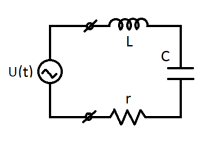
\includegraphics[scale=0.7]{../section01/images/RLC_lin/RLC_lin.png} % нужна картинка
\end{minipage} \hfill   
\begin{minipage}{10cm}
Пусть $U(t) = U_0 e^{\jo t}$ (МКА).
Раскроем напряжение по всем элементам (т.е. запишем "уравнение движения"):
$$L \dfrac{di}{dt} + i r + \dfrac{1}{C} \displaystyle \int i \, dt = U.$$
\end{minipage}

Найдём решение в виде, $i = \widetilde{i} e^{\jo t}$ и получим:
$$\widetilde{i} = \dfrac{U_0}{r + \jo L + \dfrac{1}{\jo C}} = \dfrac{U_0}{r + j (\omega L - \dfrac{1}{\omega C})} = \dfrac{U_0}{r + jX},$$
где $X = \omega L - \dfrac{1}{\omega C} = \dfrac{\omega^2 LC - 1}{\omega C}$ --- реактивная часть сопротивления контура (для $X = 0 \Rightarrow \omega~=~\omega_0~=~\dfrac{1}{\sqrt{LC}}$). Значит, при частоте $\omega = \omega_0$ ток достигает максимума $|i|_{max} = \dfrac{U_0}{r}$, т.е. амплитуда тока в контуре такова, что $L$ и $C$ как будто отсутствуют. Объясним причину этого явления.

Исследуем напряжения на индуктивности и на конденсаторе при $\omega = \omega_0$:

$$U_L = \jo L \cdot \dfrac{U_0}{r} e^{\jo t} \bigg|_{\omega = \omega_0} = \dfrac{1}{r} \sqrt{\dfrac{L}{C}} U_0 e^{j(\omega t + \dfrac{\pi}{2})}, \quad \dfrac{\omega_0 L}{r} = \dfrac{1}{r} \sqrt{\dfrac{L}{C}}$$
$$U_C = \dfrac{1}{\jo C} \cdot \dfrac{U_0}{r} e^{\jo t} \bigg|_{\omega = \omega_0} = \dfrac{1}{r} \sqrt{\dfrac{L}{C}} U_0 e^{j(\omega t - \dfrac{\pi}{2})}, \quad \dfrac{1}{\omega_0 Cr} = \dfrac{1}{r} \sqrt{\dfrac{L}{C}}$$

Получается, что напряжения $U_L$ и $U_C$ противофазны и равны по модулю, т.е. компенсируют друг друга: $U_L (\omega_0) = - U_C (\omega_0)$. Рассмотрим добротность:
$$\dfrac{\omega_0 L}{r} = \dfrac{1}{\omega_0 Cr} = \dfrac{1}{r} \sqrt{\dfrac{L}{C}} = Q,\quad ~\rightarrow~?$$
Покажем, что $Q = 2\pi \dfrac{\text{колебательная энергия в контуре}}{\text{энергия, теряемая за период}}$:
$$Q = 2\pi \dfrac{W}{P_{\text{mean}} T} = \omega_0 \dfrac{W}{P_{\text{mean}}} = \omega_0 \dfrac{\dfrac{L}{2} \bigg( \dfrac{U_0}{r} \bigg)^2}{U_0^2 / (2r)} = \dfrac{\omega_0 L}{r} = \dfrac{1}{r} \sqrt{\dfrac{L}{C}}.$$

Здесь $P_{\text{mean}}$ --- средняя за период мощность (из-за усреднения появляется деление на 2), $Q$ --- добротность контура (в английской литературе "quality factor").

Видно, что при $\omega = \omega_0 \rightarrow |U_L| = |U_C| = U_0 Q$, т.е. на реактивных элементах напряжение возрастает в $Q$ раз (именно по этой причине последовательный резонанс называется "резонансом напряжений"). Напомним: 
$$Q = \dfrac{\omega_0 L}{r} = \dfrac{1}{\omega_0 Cr}.$$
Найдём частотную характеристику $K(\jo)$:
$$\widetilde{i}(\jo) = \widetilde{K}(\jo) U(\omega), \quad \widetilde{i}(\jo) = \widetilde{I}(\omega) e^{j(\varphi(\omega) + \omega t)};$$
$$I(\omega) = |\widetilde{K}(\jo)| U_0 = \bigg| \dfrac{1}{r + jX}\bigg| U_0 = \dfrac{r}{\sqrt{r^2 + \bigg(\dfrac{\omega^2 LC - 1}{\omega C} \bigg)^2}} \cdot \dfrac{U_0}{r}.$$
Очевидно, $|I|_max = \dfrac{U_0}{r}$, при $r = \dfrac{\omega^2 LC - 1}{\omega C}$ амплитуда падает в $\sqrt{2}$ раза. Какова расстройка $(\omega - \omega_0)$ при таком сопротивлении?
$$\omega rC = \omega^2 LC - 1,~\text{введём замену } x = \dfrac{\omega}{\omega_0} \Rightarrow x^2 - \dfrac{1}{Q} x - 1 = 0;$$

\begin{minipage}{6cm}
\centering
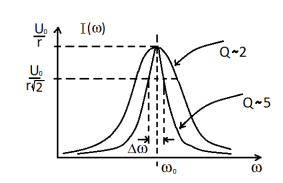
\includegraphics[scale=0.7]{../section01/images/I_o_RLC_lin/I_o_RLC_lin.png} % нужна картинка
\end{minipage} \hfill   
\begin{minipage}{10cm}
Решением этого уравнения будут:
$$x = \dfrac{1}{2Q} \pm \sqrt{1 + \dfrac{1}{4 Q^2}} \simeq  \dfrac{1}{2Q} \pm \bigg( 1 + \dfrac{1}{2 Q^2}\bigg) = \dfrac{\omega_0 \pm \delta \omega}{\omega_0}.$$
Данное приближение верно при $Q \gg 1$. Тогда, полная ширина на "полувысоте"{} (корректнее, на $1/\sqrt{2}$ высоты): $\Delta \omega = 2\delta \omega$ и $Q = \dfrac{\omega_0}{\Delta \omega}$. Таким образом мы получили ещё один способ нахождения добротности по ширине резонансной кривой.
\end{minipage}

\begin{minipage}{6cm}
\centering
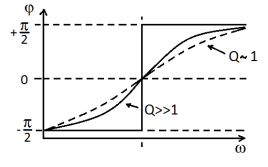
\includegraphics[scale=0.7]{../section01/images/phi_o_RLC_lin/phi_o_RLC_lin.png} % нужна картинка
\end{minipage} \hfill   
\begin{minipage}{10cm}
Исследуем поведение фазовой кривой:
\begin{itemize}
\item При $\omega \rightarrow 0$ виден ёмкостный характер импеданса (ток бежит "вперёд"{} напряжения).
\item При $\omega = \omega_0$ импеданс чисто активный.
\item При $\omega \rightarrow \infty$ виден индуктивный характер импеданса (ток "отстаёт"{} от напряжения).
\end{itemize}
\end{minipage}
Общий вид зависимости фазы от частоты:
$$\tan \varphi = \dfrac{\omega^2 LC - 1}{\omega rC} = \dfrac{x^2 - 1}{x} \cdot Q.$$
Значит, при $Q \rightarrow \infty$, $\varphi(\omega)$ приближается к "ступеньке"{} и такой контур называется "идеальным".

\subsection{Параллельный колебательный контур.}

\begin{minipage}{6cm}
\centering
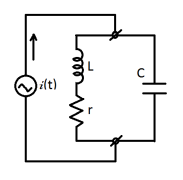
\includegraphics[scale=0.7]{../section01/images/RLC_par/RLC_par.png} % нужна картинка
\end{minipage} \hfill   
\begin{minipage}{10cm}
Пусть $Z(\jo)$ --- импеданс контура.
$$\dfrac{1}{Z} = \jo C + \dfrac{1}{r + \jo L},\quad Z = \dfrac{r + \jo L}{(1 - \omega^2 LC) + \jo rC}.$$
При $r = 0$ (т.е. в случае "идеального"{} контура), $Z$ имеет максимум при $\omega = \omega_0 = \dfrac{1}{\sqrt{LC}}$ (и ток во внешней цепи минимален).

При $r \neq 0$, но с $Q \gg 1$, максимум сдвигается на $\delta \omega$:
\end{minipage}
$$\delta \omega = \omega_{\text{рез}} - \omega_0 ~(\text{здесь } \omega_{\text{рез}} \equiv \omega_{max}),~\text{причём}~\boxed{\dfrac{\delta \omega}{\omega_0} \simeq -\dfrac{1}{2 Q^2}}$$
\textbf{Упражнение 4.} Докажите последнее соотношение.

На резонансной частоте $\omega_{\text{рез}} = \omega_0 + \delta \omega \simeq \omega_0$ импеданс контура равен:
$$|Z| = \bigg( \dfrac{r^2 (1 + Q^2)}{(1 - \omega^2 LC)^2 - 1/Q^2} \bigg)^{1/2} \bigg|_{\omega=\omega_{\text{рез}} \sim \omega_0} \simeq Q^2 r.$$

Таким образом, на резонансе сопротивление параллельного контура возрастает в $Q^2$ раз, по сравнению с собственным активным сопротивлением! Какого поведение токов в ветвях контура?

Падение напряжения на контуре $U = Z i_0$, где $i_0$ идёт с генератора тока:
\begin{equation*}
 \begin{cases}
   i_C |_{\omega \sim \omega_0} = \dfrac{r Q^2}{1/(\jo_0 C)} i_0 = \jo_0 rC Q^2 i_0 &= Q i_0 e^{j \dfrac{\pi}{2}} \\ 
   i_L |_{\omega \sim \omega_0} = \dfrac{r Q^2}{\jo_0 L} i_0 \Rightarrow &= Q i_0 e^{-j \dfrac{\pi}{2}}
 \end{cases}
\end{equation*}

Отсюда видно, что токи ветвей увеличились в $Q$ раз, но они противофазны, поэтому ток во внешней цепи мал. Данное явление называется "резонансом токов".

Для $Q \rightarrow \infty$  контур имеет $r\rightarrow 0$ и тока во внешней цепи нет, т.е. источник можно отключить! % или сопротивление стремится к бесконечности?

Исследуем фазовую характеристику: 
$$\widetilde{U} = i \widetilde{Z}(\jo), \quad \tan\varphi = \dfrac{\text{Im} \widetilde{Z}}{\text{Re}\widetilde{Z}}$$
Перепишем импеданс в форме:
$$\widetilde{Z} = \dfrac{(r + \jo L) \cdot \dfrac{1}{\jo C}}{(r + \jo L) + \dfrac{1}{\jo C}} \simeq [r \ll \omega L \Rightarrow Q \gg 1] \simeq \dfrac{L/C}{r + j(\omega L - \dfrac{1}{\omega C})} \Rightarrow \boxed{\tan \varphi = Q \bigg[ \dfrac{\omega}{\omega_0} - \dfrac{\omega_0}{\omega}\bigg]}$$
\textbf{Упражнение 5.} Постройте график $\varphi(\omega)$, причём:
\begin{itemize}
\item Слева от резонанса $\omega < \omega_0$, $\varphi \rightarrow -\dfrac{\pi}{2}$ при $\omega \rightarrow 0$ (ёмкостный характер импеданса);

\item Справа от резонанса $\omega > \omega_0$, $\varphi \rightarrow \dfrac{\pi}{2}$ при $\omega \rightarrow \infty$ (индуктивный характер импеданса).
\end{itemize}

\subsection{Осциллятор в радиофизике.}

Колебательные контуры в \textit{п.8 и п.9} это частные случаи очень важного "элементарного звена"{} в радиофизике и в физике вообще. По этой причине его свойства следует знать досконально. Общепринятая терминология --- "осциллятор". Линейный осциллятор описывается дифференциальным уравнением второго порядка.

Для колебательного контура мы имели: $L \dfrac{di}{dt} + i r + \dfrac{1}{C} \displaystyle \int i \, dt = U$, вводя замену $q = \dfrac{di}{dt}$ или после дифференцирования мы получим уравнение в стандартной форме:
$$i'' + 2\delta i' + \omega_0^2i = f(t),$$
где $\delta = \dfrac{r}{2L}$ --- показатель затухания, $\omega_0$ --- собственная частота и $f(t) \rightarrow \dfrac{U'(t)}{L}$ --- внешнее воздействие. 

Большой класс измерительных приборов, например, акселерометр, гравиметр, сейсмограф и др., имеют в качестве основного рабочего элемента осциллятор в виде упругой закрепленной массы.

\begin{minipage}{6cm}
\centering
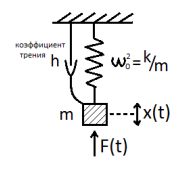
\includegraphics[scale=0.7]{../section01/images/oscillator/oscillator.png} % нужна картинка
\end{minipage} \hfill   
\begin{minipage}{10cm}
Уравнение движения для $x(t)$ в стандартной форме это тоже самое с заменой:
$$\delta = \dfrac{R}{2L} \rightarrow \dfrac{h}{2m}$$
$$\omega_0 = \dfrac{1}{\sqrt{LC}} \rightarrow \sqrt{\dfrac{k}{m}}$$
$$Q = \dfrac{1}{r} \sqrt{\dfrac{L}{C}} \rightarrow \dfrac{1}{h} \sqrt{km}$$
\end{minipage}
Получаем $x'' + 2\delta x' + \omega_0^2x = f(x), f(x) = \dfrac{F(x)}{m}.$

Осциллятор (также как простейшие $RC$- и $RL$-цепочки) --- инерционный элемент. Его характерное время релаксации $\tau^* = 1/\delta = 2Q/\omega_0$.

Явление резонанса в \textit{п.8, п.9} описано как стационарный (установившийся) процесс с характерными чертами. Инерционность обуславливает наличие также нестационарных (или "переходных") процессов в поведении осциллятора. Расчет переходных режимов нельзя провести методом К.А.; подходит метод преобразования Лапласа \textit{п.7}. В радиофизике часто используют также "метод медленно меняющихся амплитуд"(ММА).

\subsection{Метод ММА --- в гармоническом приближении.}

\subsection{Линейные четырёхполюсники.}

\subsection{Связанные колебательные контуры.}
\end{document}
